\documentclass[a4paper]{article}

%% Language and font encodings
\usepackage[english]{babel}
\usepackage[utf8x]{inputenc}
\usepackage[T1]{fontenc}

%% Sets page size and margins
\usepackage[a4paper,top=3cm,bottom=2cm,left=3cm,right=3cm,marginparwidth=1.75cm]{geometry}

%% Useful packages
\usepackage{amsmath}
\usepackage{graphicx}
\usepackage{subcaption}
\usepackage[colorinlistoftodos]{todonotes}
\usepackage[colorlinks=true, allcolors=blue]{hyperref}

% http://www.tablesgenerator.com/#
\usepackage[normalem]{ulem}
\useunder{\uline}{\ul}{}

\title{Classification of folktales}
\author{Dominik Macháček, Martin Banzer}

\begin{document}
\maketitle



\section{Introduction}
In this paper we contribute to folkloristic research by designing an
automatic classifier of texts according to Aaarne-Thompson-Uther (ATU)
classification system, which was developed as a standardized way for
organization of texts for folkloristics research. With a support of our automatic classifier,
researchers can easier study real-world stories transmission and origin.
In our work we used the annotated
corpus of texts from the Multilingual Folk Tale Database \cite{mftd}. Our work also includes a crawler for downloading this corpus from the Internet.
%TODO: our best accuracy result?
%TODO: which approach we used -- supervised machine learning


\section{Corpus description}

\subsection{Aarne-Thompson-Uther index}


\begin{figure}
\centering
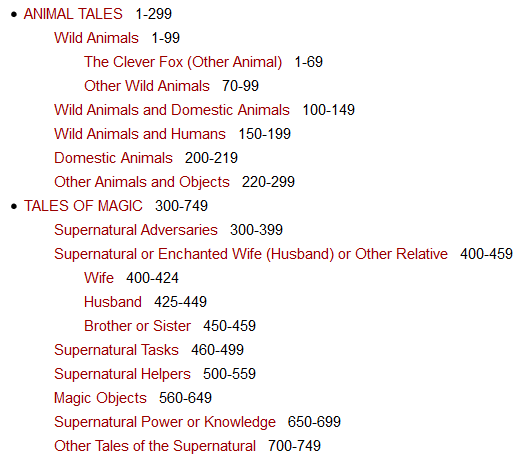
\includegraphics[width=0.9\linewidth]{random/ATU.PNG}
%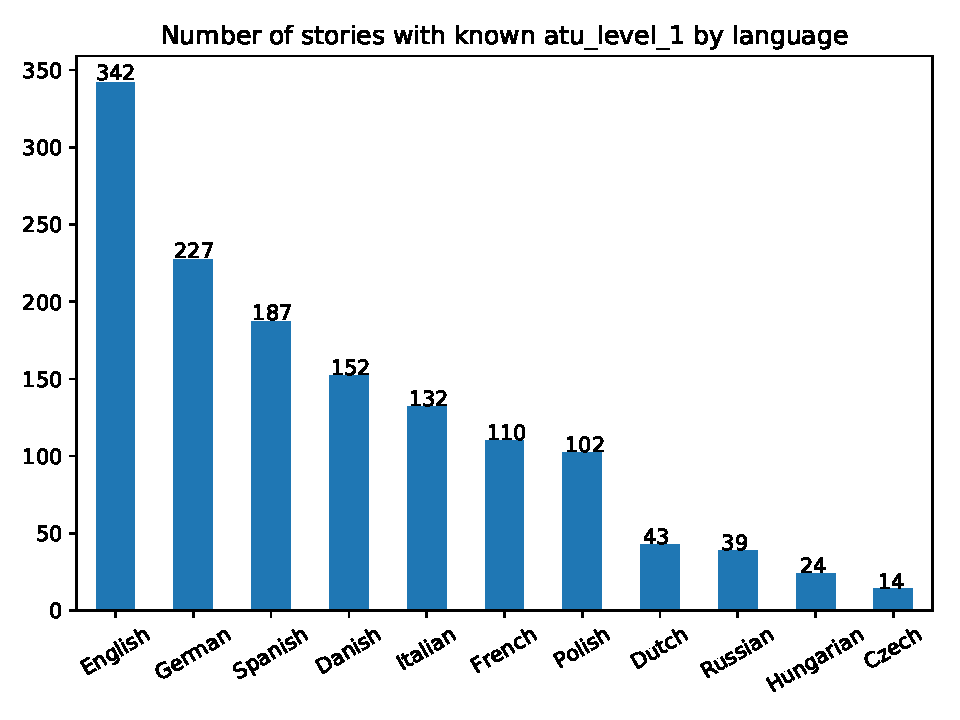
\includegraphics[width=0.9\linewidth]{plots/bars2.pdf}
\caption{Example of the classification levels from the ATU. \textit{ANIMAL TALES} and \textit{TALES OF MAGIC} are in the first level, \textit{Wild Animals, Wild Animals and Domestic Animals} and \textit{Wild Animals and Humans} are in the second level and \textit{The Clever Fox} and \textit{Other Wild Animals} are in the third level. The numbers behind each line are so called ATU numbers which belong to each category. They are irrelevant for our work.}
\label{fig:atu}
\end{figure}

In the Aarne-Thompson-Uther index (ATU), folktales are divided into 7 groups: animal, magic, realistic, stupid ogre, anecdotes and jokes, formula. These labels are in so called ATU-level-1.

These groups are then subdivided into another groups, as figure \ref{fig:atu} shows.




\subsection{Multilingual Folk Tale Database}
The Multilingual Folk Tale Database (MFTD) \cite{mftd} is a collection of folktales that provides for each tale information about its title, language and ATU group.
Since there is no reliable folktale classifier yet, every tale has to be assigned to one of the ATU groups manually by experts. 
MFTD is open database, everyone can create an account, upload
stories to MFTD and label them, even if he or she is actually not an expert. Therefore some of the labels might be disputable. In all groups there is an \textit{other} section, which contains the most questionable tales.
Also there are some tales which have no label at all.
We collected those tales in a group called \textit{Unknown}.

\subsection{Crawler}

Our colleague Simon Ahrendt provided us with a crawler that covered the Multilingual Folktale Database and extracted folktales with available metadata. This gave us an access to information about the language, the ATU index number and title.

Special acknowledgments to Simon.

\subsection{Distribution of languages and labels}

The Multilingual Folk Tale Database contains stories in 11 languages. We
crawled all of them. Figure \ref{fig:bar1} summarizes the number of stories
by language. In total we have 901 stories in English and between roughly 500
and 600 stories in other 4 languages, French, Spanish, Hungarian and
Russian. We realized we have too few stories in German, Danish, Polish,
Italian, Czech and Dutch to make a strong supervised classifier for them.

We also realized that most of stories in our Multilingual Folk Tale
Database don't have ATU labels assigned. Figure \ref{fig:bar2} shows the
numbers of stories with known ATU level 1 by languages.
The language with most labeled stories is English, we have 342 labeled
stories. The second is German with 227 stories. This is too few for
supervised classifier, therefore we decided to focus our work only to
English stories. For other languages we have too few resources.

% https://en.wikibooks.org/wiki/LaTeX/Floats,_Figures_and_Captions
\begin{figure}
\centering
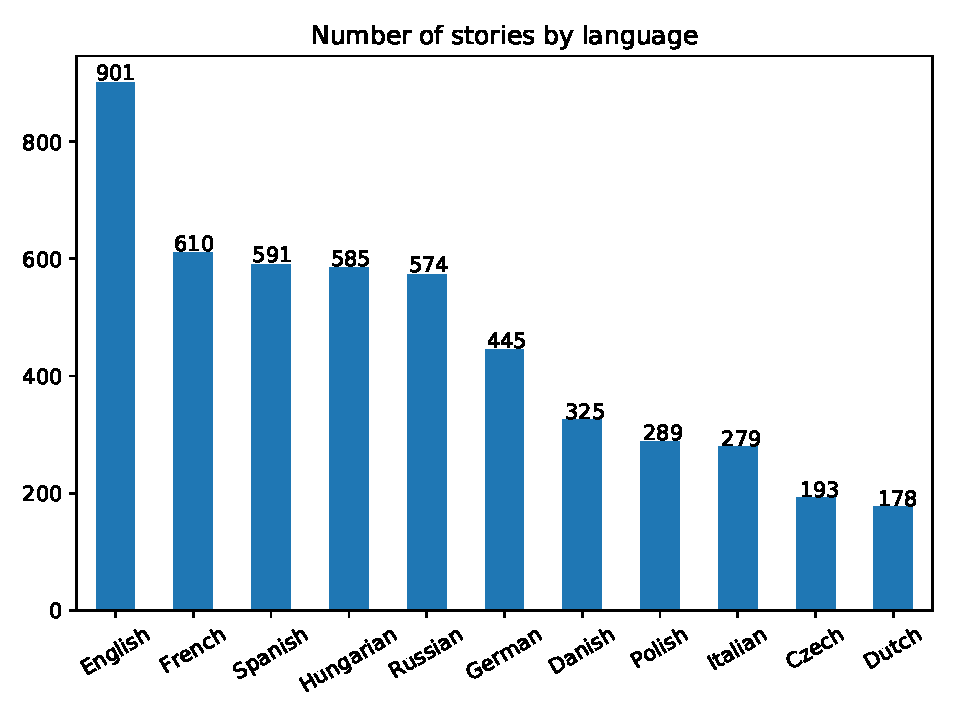
\includegraphics[width=0.9\linewidth]{plots/bars1.pdf}
%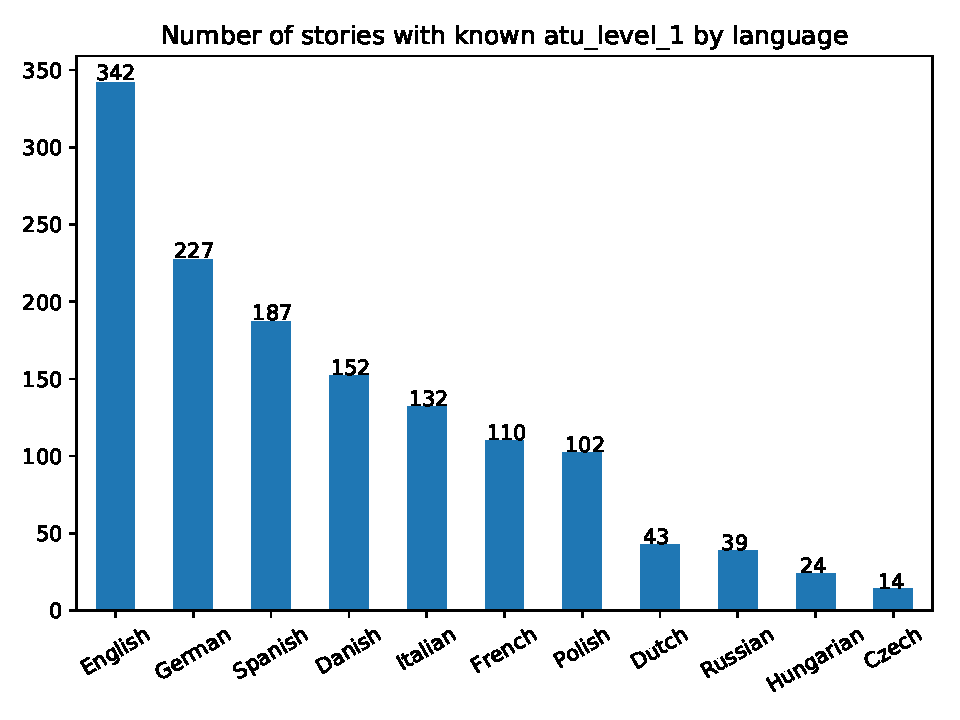
\includegraphics[width=0.9\linewidth]{plots/bars2.pdf}
\caption{Number of all stories by language.}
\label{fig:bar1}
\end{figure}

\begin{figure}
\centering
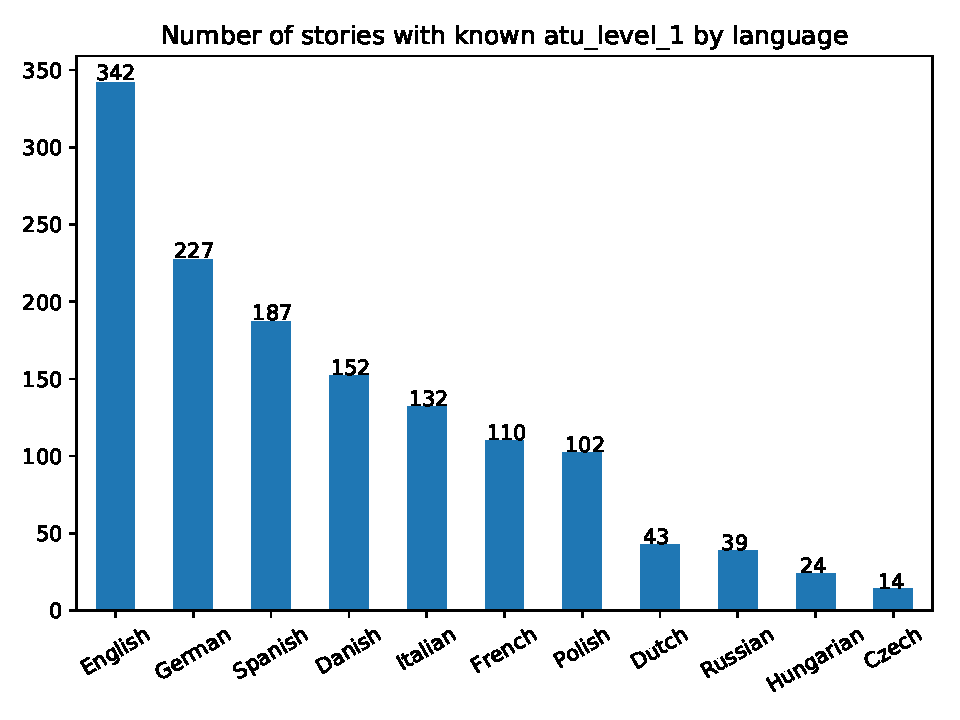
\includegraphics[width=0.9\linewidth]{plots/bars2.pdf}
\caption{Number of stories with known ATU level 1 by language.}
\label{fig:bar2}
\end{figure}

Next we focused on the distribution of labels of English stories by level
1 and 2. Figure \ref{fig:bar3} shows that we have 7 classes by level 1:
176 Tales of Magic, 78 Animal Tales, 46 Anecdotes and Jokes. We have 14, 12,
7 and 7 representatives of other four classes.

Figure \ref{fig:bars} describes the distribution of stories by level 2. We
realized we have too few representatives of most classes by level 2, therefore
we decided to focus only on level 1.

\begin{figure}
\centering
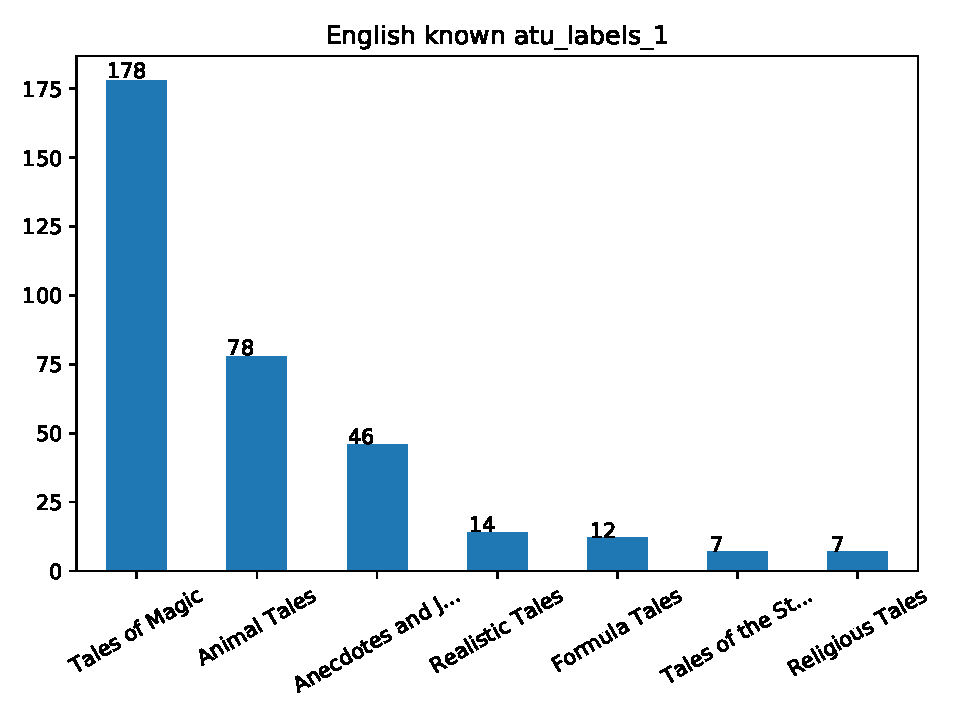
\includegraphics[width=0.9\linewidth]{plots/bars3.pdf}
\caption{Distribution of English stories by ATU level 1.}
\label{fig:bar3}
\end{figure}

\begin{figure} \centering
\begin{subfigure}{.5\textwidth}
\centering
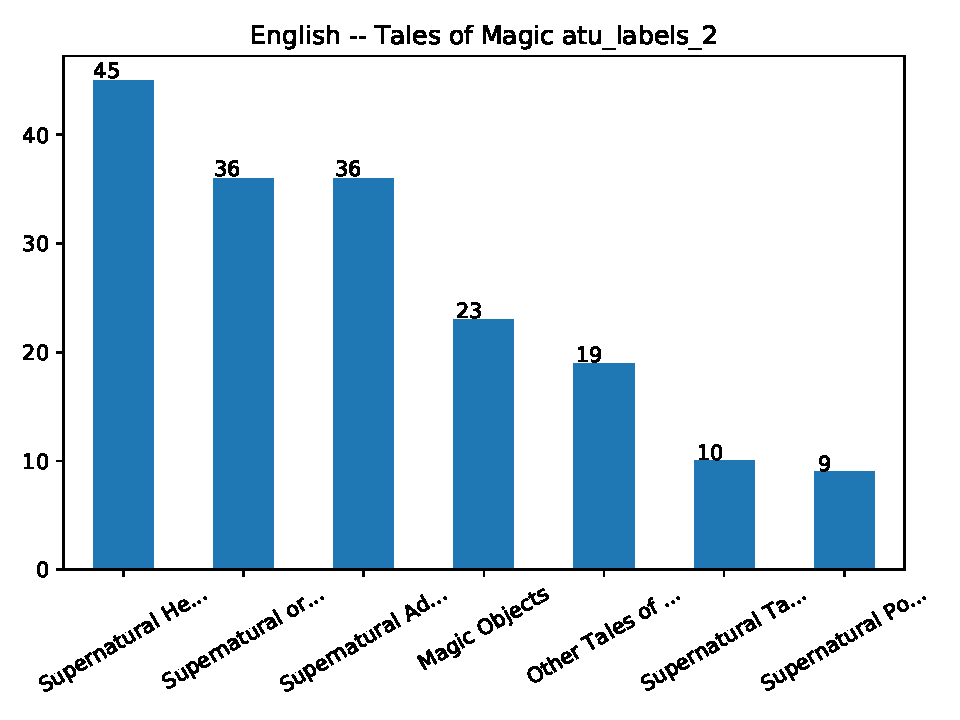
\includegraphics[width=0.9\linewidth]{plots/bars10.pdf}
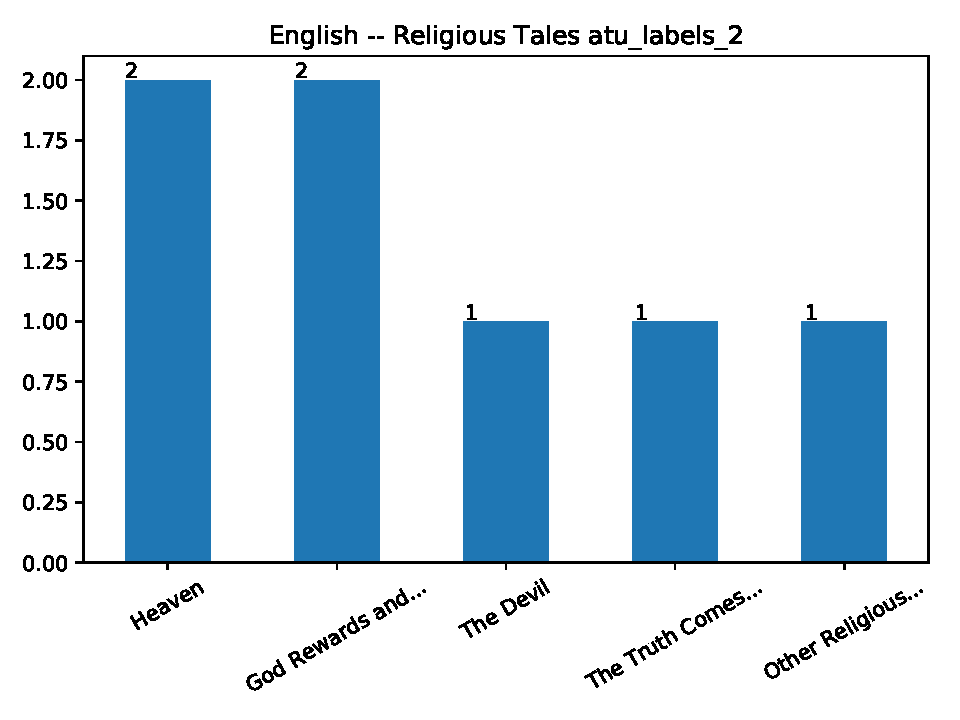
\includegraphics[width=0.9\linewidth]{plots/bars4.pdf}
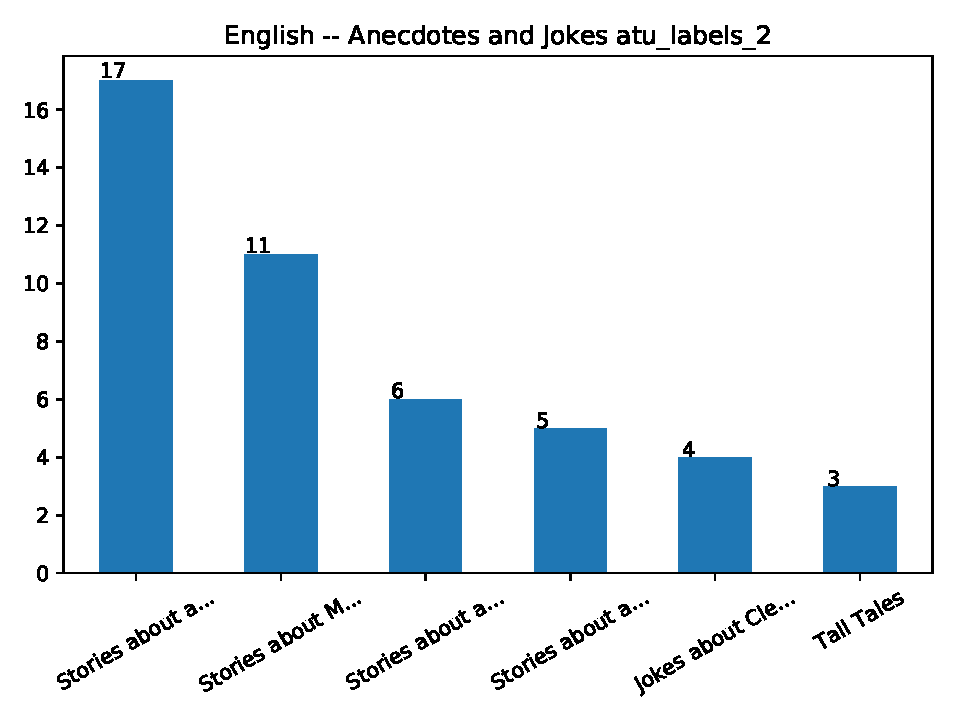
\includegraphics[width=0.9\linewidth]{plots/bars6.pdf}
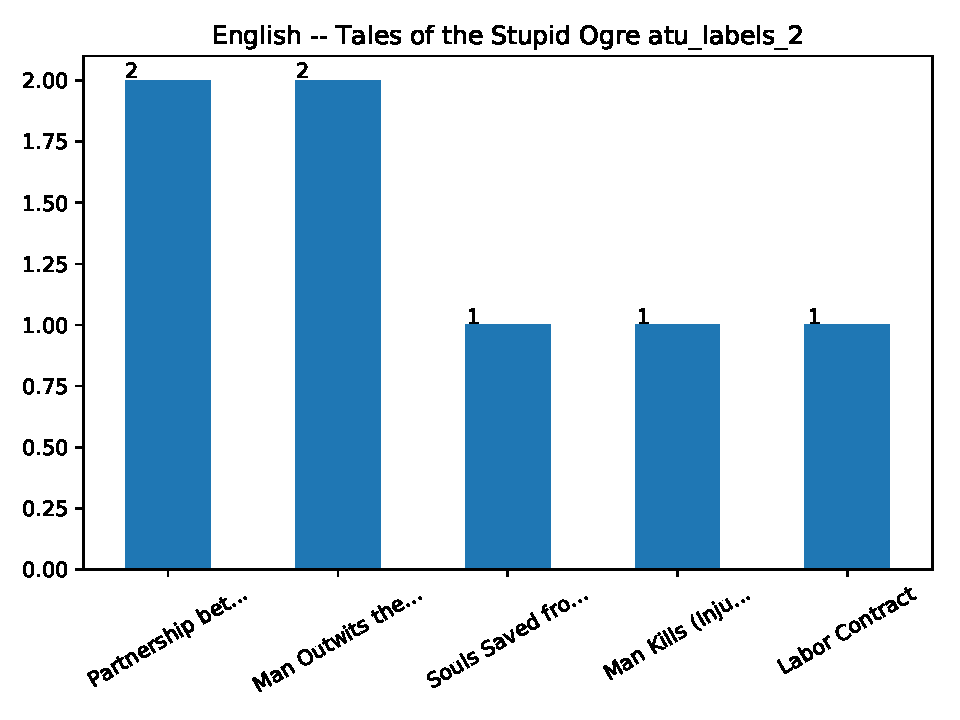
\includegraphics[width=0.9\linewidth]{plots/bars7.pdf}
\end{subfigure}%
\begin{subfigure}{.5\textwidth}
\centering
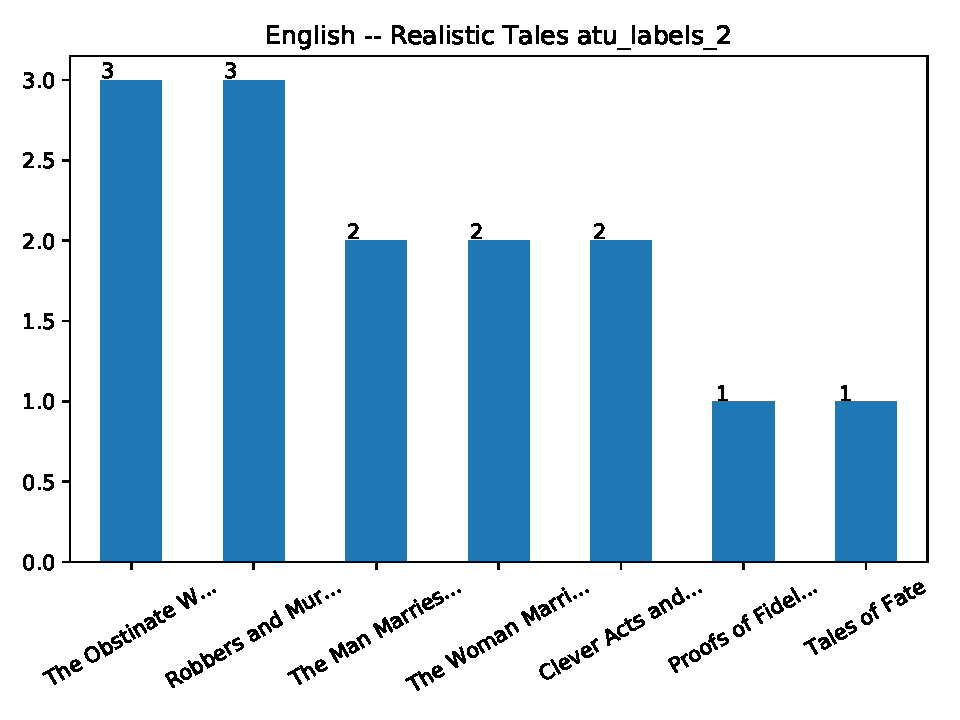
\includegraphics[width=0.9\linewidth]{plots/bars8.pdf}
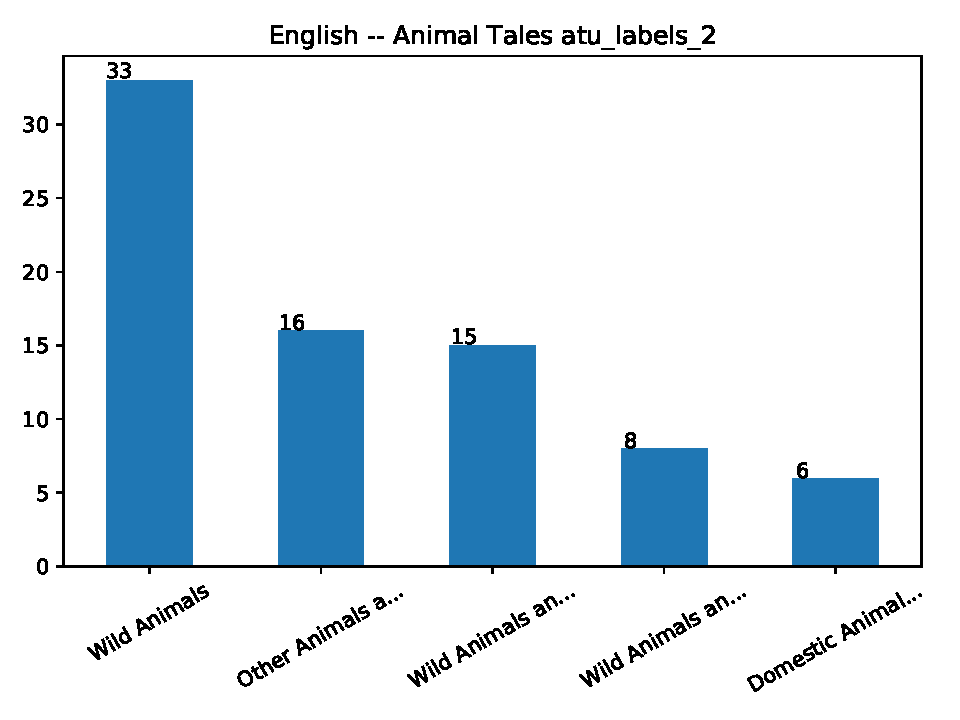
\includegraphics[width=0.9\linewidth]{plots/bars9.pdf}
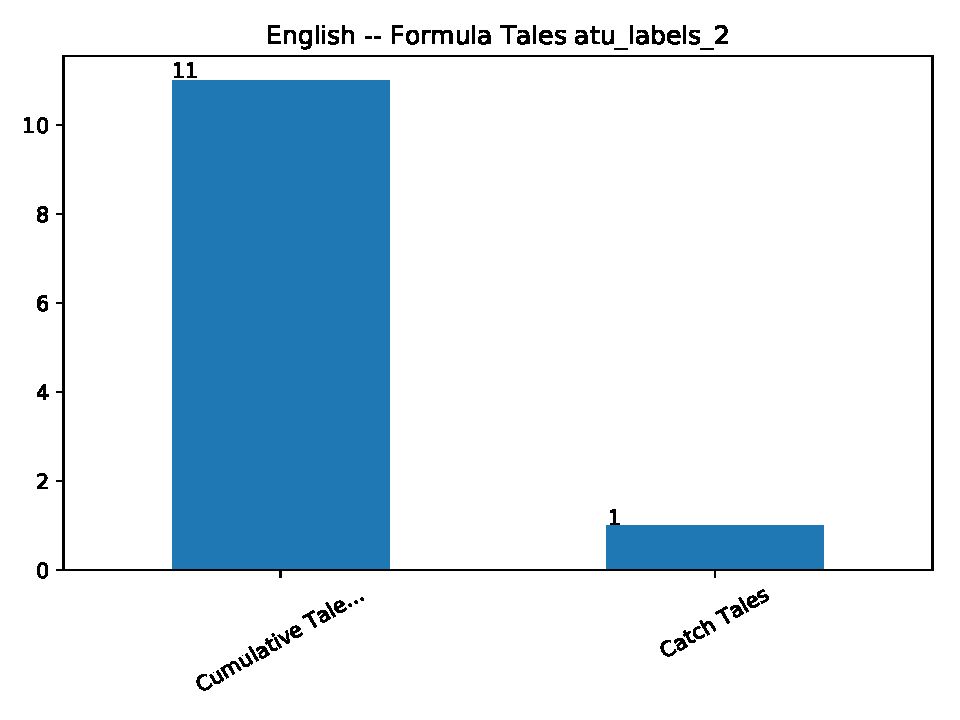
\includegraphics[width=0.9\linewidth]{plots/bars11.pdf}
\end{subfigure}%
\caption{Distribution of English stories by ATU level 2.}
\label{fig:bars}
\end{figure}


\section{Data preprocessing}

We split our labeled data to training and evaluation part in ratio
70:30. We made sure that the distribution of classes is the same in both parts.

Then we tokenized all texts with usage of tokenization function from NLTK
\cite{NLTK} and we removed punctuation and stopwords. 

\section{Feature design}

We designed, implemented and compared several methods for classification.

\subsection{Trivial keyword extraction}

We created two different keywordlists: one for the tale titles and the other for the actual texts.

As an example for our keywordlist creation, we will have a look at animal tales and focus on the tales texts.
For this example we computed one list, which counts the appearances of every word from every animal tale.
The other list counts the appearances of every word from every tale but the animal tales.
Finally we delete every entry from the first list which appears more often in the second list than in the first list.

\begin{figure}
\centering
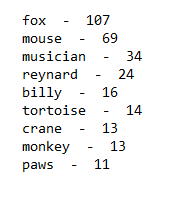
\includegraphics[]{random/sortedtextkeywords.PNG}
\caption{The most common animal tale keywords from the texts.}
\label{fig:sortkw}
\end{figure}

Figure \ref{fig:sortkw} shows the most common keywords from animal tale texts.
After we computed keywordlists for every ATU group, we noticed that some lists can be replaced by more intuitive features. For the animal tales example we could also use a list of animal names.
We tried this by specifically looking for \textit{animals} using the
% which NLTK module? which method?
NLTK WordNet module for Python. But this method also interprets the word \textit{Queen} as an animal because \textit{Queen} appears in the NLTK feature list for animals like \textit{ant queen} or \textit{bee queen}. Therefore we stayed with our keywords.

The keywordlists for the titles proved to be more problematic
because the available data is small, due to the fact that every story has
only one title and that those titles are very short, the keywordlists for
% effective -- how did you evaluate it?
% we can say that we want to classify texts with missing titles so we don't
% want to use them
titles are not as effective as the keywordlists for texts. Figure
\ref{fig:sortart} shows the most common keywords from animal tale titles.

\begin{figure}[h]
\centering
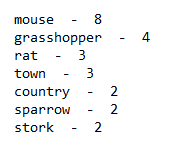
\includegraphics[]{random/sortedtitlekeywords.PNG}
\caption{The most common animal tale keywords from the texts.}
\label{fig:sortart}
\end{figure}


\subsection{Information retrieval based keyword selection}

Another approach we used was related with tf-idf statistics which is used
to reflect the importance of a term in a document with respect to another
documents. However, we can't use it because our goal is different. We
intend to find terms appearing in all (or at least in much as possible)
tales in a class and not appearing in other classes. Therefore we
implemented following statistics: 

Let $C$ be a total number
of occurrences of a term in one class and $D$ the the number of
documents in a class containing the term. The statistics we used is then  
$C^D$. We select the terms with the highest $C^D$. This emphasize terms
appearing in many tales in a class, but still gets a chance to frequent
terms to be ranked higher.

For every class we selected top 100 words by this statistics and excluded
singletons. Then we made union of these words. 

This method selects all important keywords but it also
words appearing in all categories which are useless for classification.
Therefore we later used greedy forward selection to find the best subset of
these keywords.


\subsection{Other features}

Besides the keywords we also used a list of features which simply
% which things? 
count multiple things in every ATU group.
We counted for each ATU group the amount of sentences and words, the number of proper names, the number of direct speeches and the number of special signs for texts or for titles. % this is dependent on our training data. In fact, the number of direct speeches or special signs doesn't rely on the category at all, it's obvious this can't help. It gets poor result.

In the following examples we included a special group called \textit{other stories}. These stories are non-animal stories. Thereby we can compare animal tales to \textit{other stories} which tells us for example, that on average, the length of animal tales is about a quarter of the length of other tales. % with average you can't judge whether it's good or bad feature for classification. 

Folgert Karsdorp \cite{RETELLING} discusses this topic as well. There are similar results mentioned as we got from our feature inclusion. 

% these figures are not mentioned anywhere, use \ref{fig:rand1} to reference them
\begin{figure}
\centering
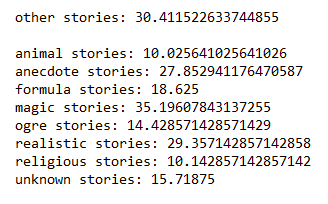
\includegraphics[]{random/directspeechtext.PNG}
% is it average? then write it
\caption{The average number of direct speeches per text in the ATU-index groups.}
% label for every figure must be unique!
\label{fig:rand1}
\end{figure}

\begin{figure}
\centering
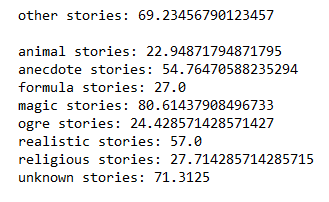
\includegraphics[]{random/sentencestext.PNG}
\caption{The average amount of sentences per text in the ATU-index groups.}
\label{fig:rand2}
\end{figure}

\begin{figure}
\centering
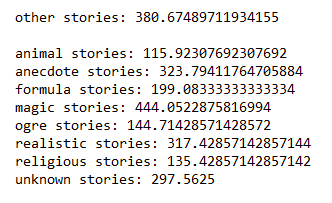
\includegraphics[]{random/specialsignstext.PNG}
\caption{The average number special signs per text in the ATU-index groups.}
\label{fig:rand3}
\end{figure}

\begin{figure}
\centering
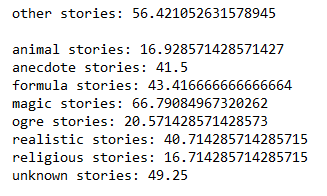
\includegraphics[]{random/propernames_text_.PNG}
\caption{The average number proper names per text in the ATU-index groups.}
\label{fig:rand4}
\end{figure}

\begin{figure}
\centering
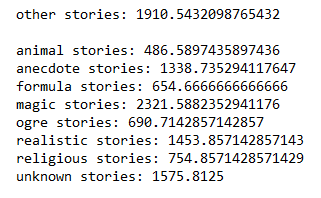
\includegraphics[]{random/wordstext.PNG}
\caption{The average amount of words per text in the ATU-index groups.}
\label{fig:rand5}
\end{figure}

\begin{figure}
\centering
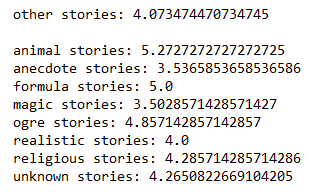
\includegraphics[]{random/wordstitle.PNG}
\caption{The average amount of words per title in the ATU-index groups.}
\label{fig:rand6}
\end{figure}


%\subsection{Evaluation}
%
%% Please, elaborate more. I'd also like to see the code you computed it with. And which classifier? 
%We tested our features with a classifier, that checked for some tales, which features are fulfilled and also how good those features got matched.
%We achieved a accuracy of about 80\% for each ATU-index group.
%The classifier also failed to classify some stories. 
%% Do you mean you read the story and found out it's incorrectly labeled? Then write it.
%As it turns out, several of the \textit{incorrectly} classified stories were from the \textit{other} section within the ATU-index groups.
%This means that their initial assignment to their ATU-index group was already questionable.
%


\subsection{Summary of feature selection}

Here we summarize all feature selection methods we implemented and
compared. Numbers with hashtag are used as a reference to table with
evaluation results.

\begin{verbatim}
#1.0 simple most frequent words
-- take 20 mfw for each category
-- values are numbers of occurences in a text
-- not scaled

#1.1
-- same as #1, but 
-- MinMaxScaling were used
-- not total number of occurences in a text, but number of occ/text
length
		    
#2.0
-- take 100 words by highest value of C^D
   -- C is a total number of occurences in all text in a class
   -- D is a number of documents in a class containing given word
   -- ^ is power
-- don't remove words chosen from 2 classes
-- in total, 242 words
-- scaled

#2.1
-- order features by forest features importance
-- use greedy forward selection to find optimal number of features -- it's 14
		    
#2.2
-- use binary features, not real
    -- 0 or 1: keywords appears at least once in a text
    -- new forward selection
    -- optimal number is 16
\end{verbatim}

\section{Classification}

In previous section we elaborated several methods for design of features.
Here we describe the actual classification and evaluation.

\subsection{Feature values}

Once we have a list of typical words for every category, we have to create
a feature matrix. Its rows are the documents and columns are the keywords. 
We implemented and compared several methods how to fill the matrix values.
The values can be the absolute numbers of occurrences of given word in
a document. One high value can unbalance the whole classifier, so second
option is to scale them to [0,1]-range using min-max scaling. And the third option is
to use only binary values zero or one: one if the word appears in the
document at least once, zero otherwise.

With these matrices we trained several classifiers from \texttt{sklearn}
library and evaluated their performance on test set. 

Our comparison shows that the binary values give the best performance.

%\subsection{Greedy forward selection}
%





\subsection{Classification evaluation results}

We used several classification methods from \texttt{scikit} library: K-NN,
SVM, Decision Tree, Random Forest, AdaBoost and Naive Bayes. We used them
with different parameters to find the best settings.

Table \ref{tab:7class} summarizes the best results from 7-class
classification, it is a problem where one correct label from all 7 classes
has to be assigned. It shows that feature set \#2.2 is the best, the
accuracy with Linear SVM classifier is 78\%. Baseline is 51\%, it is the
accuracy which can be achieved by predicting the most frequent class in all
cases.

\begin{table}[h]
\centering
\begin{tabular}{|l|l|l|}
\hline
\multicolumn{1}{|c|}{\textbf{feature set}} & \multicolumn{1}{c|}{\textbf{classifier}} & \textbf{accuracy} \\ \hline
 & baseline & 0.51 \\ \hline
\#1.0 & SVM & 0.71 \\ \hline
\#1.1 & Decision Tree & 0.6777 \\ \hline
\#2.1 & Random Forest & 0.7333 \\ \hline
\#2.2 & Linear SVM & {\ul \textbf{0.7778}} \\ \hline
\end{tabular}
\caption{Evaluation results of 7-class classification.}
\label{tab:7class}
\end{table}

Furthermore, we did also binary classification for 3 most frequent classes
because for other classes we have too few resources. The results are in
table \ref{tab:an}, \ref{tab:jokes} and \ref{tab:magic}.

\begin{table}[h]
\centering
\begin{tabular}{|l|l|l|}
\hline
\multicolumn{1}{|c|}{\textbf{feature set}} & \multicolumn{1}{c|}{\textbf{classifier}} & \textbf{accuracy} \\ \hline
 & baseline & 0.7444 \\ \hline
\#2.2 & AdaBoost & {\ul \textbf{0.9333}} \\ \hline
\end{tabular}
\caption{Evaluation results of binary classification, Animal Tales vs.
others.}
\label{tab:an}
\end{table}

\begin{table}[h]
\centering
\begin{tabular}{|l|l|l|}
\hline
\multicolumn{1}{|c|}{\textbf{feature set}} & \multicolumn{1}{c|}{\textbf{classifier}} & \textbf{accuracy} \\ \hline
 & baseline & 0.8667 \\ \hline
\#2.2 & AdaBoost & {\ul \textbf{0.9111}} \\ \hline
\end{tabular}
\caption{Evaluation results of binary classification, Anecdotes and Jokes vs.
others.}
\label{tab:jokes}
\end{table}

\begin{table}[h]
\centering
\begin{tabular}{|l|l|l|}
\hline
\multicolumn{1}{|c|}{\textbf{feature set}} & \multicolumn{1}{c|}{\textbf{classifier}} & \textbf{accuracy} \\ \hline
 & baseline & 0.5111 \\ \hline
\#2.2 & AdaBoost & {\ul \textbf{0.8889}} \\ \hline
\end{tabular}
\caption{Evaluation results of binary classification, Tales of Magic vs.
others.}
\label{tab:magic}
\end{table}



\section{Annotation validation}

Since our corpus was annotated by anonym, we decided to    implement a test for validity of annotation, attempt to find incorrectly or disputably labeled stories and suggest experts to revise them.

We tried two approaches, clustering and leave-one-out cross-validation with cosine similarity.

For both tests we stemmed the texts and removed punctuation and stopwords. Then we created a vector of absolute frequencies of remaining terms for every document. 

\subsection{Clustering for annotation validation}

We used a linkage clustering algorithm with cosine similarity as a similarity measure. We applied it to test set and plotted its result as a dendrogram, see figure \ref{fig:dend}. The algorithm found 2 big clusters. The yellow cluster consists mostly of Magic tales, but some Magic tales appear in other clusters, and some tales, for example animal tale \textit{The Way Of The World}, appear to be more similar to Magic tales than to other animal tales. Maybe it's incorrectly annotated, maybe it's only an coincidence. We suggest experts to revise all such stories.

\begin{figure}
\centering
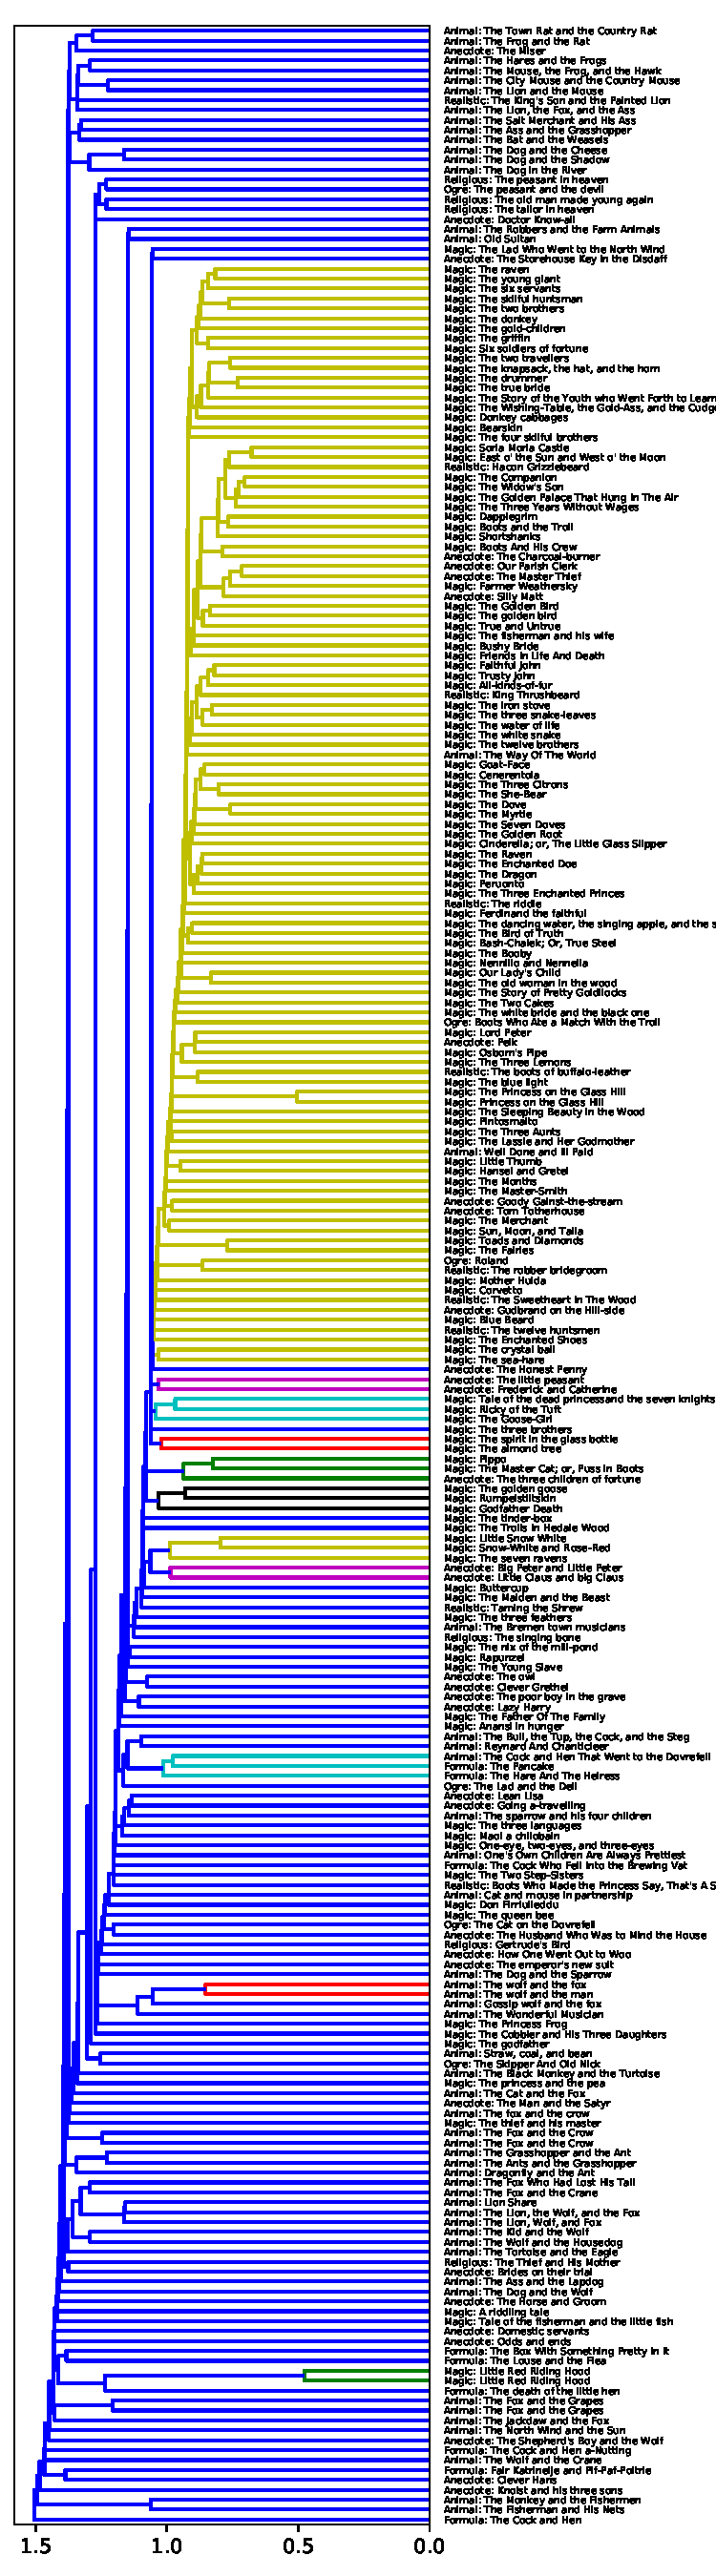
\includegraphics[height=0.9\textheight]{plots/dendrogram.pdf}
\caption{Dendrogram from linkage clustering algorithm. Branch colors represent automaticaly created clusters from clustering algorithm. In branch labels are actual labels and story titles.}
\label{fig:dend}
\end{figure}

\subsection{Leave-one-out cosine similarity}

With the second test we implemented we attempt to judge a coherence of the actual labeling to classes in training data. For every class and every story in a class, we counted the average cosine similarity to all other stories in the class. Then we printed the result as found outliers. As an outlier we used the inter-quartile range method, outliers are the elements appearing outside the interval $(Q_1 - 1.5 |Q_1-Q_3|, Q_3 + 1.5 |Q_1-Q_3| )$, where $Q_1$ is the value of first quartile and $Q_3$ the third quartile.

According to this test, all stories but 3 appear to be correctly assigned. The outliers are summarized in figure \ref{fig:outliers}. 

Futhermore, we made a 7-class classifier returning a class with the lowest average cosine similarity to training stories. We evaluated it on test set. Its accuracy was 46.67 \%, which is below a baseline 51 \%. This method is not optimal for classification.

\begin{figure}
\centering
\begin{verbatim}
Format description:
average_cosine_similarity    story_id      story_title



Realistic Tales:
0.2548	5518 The King's Son and the Painted Lion
--------- IQR lower bound: 0.3020 -------- 
0.3801	3249 Boots Who Made the Princess Say, That's A Story
==== First quartile ====
0.3824	3261 Taming the Shrew
0.3886	3305 The Sweetheart In The Wood
0.4123	1885 The boots of buffalo-leather
==== Median ===
0.4164	383 The robber bridegroom
0.4218	640 The twelve huntsmen
==== Third quartile ====
0.4360	212 The riddle
0.4495	498 King Thrushbeard
0.4546	3248 Hacon Grizzlebeard
--------- IQR upper bound: 0.5164 -------- 

Tales of Magic:
0.1629	1529 A riddling tale
0.2143	4020 Tale of the fisherman and the little fish
--------- IQR lower bound: 0.2246 -------- 
0.2281	249 Little Red Riding Hood
0.2301	3355 Little Red Riding Hood
0.2388	2015 The princess and the pea
0.2402	649 The thief and his master
0.2517	402 The godfather
0.2556	8096 Maol a chliobain
0.2771	1237 One-eye, two-eyes, and three-eyes
...
\end{verbatim}
\caption{All possibly incorrectly annotated tales found by leave-one-out cosine similarity test.}
\label{fig:outliers}
\end{figure}




\nocite{*}
\bibliographystyle{alpha}
\bibliography{bibliography}

\end{document}
